\section{Introducere}

\begin{summary}
  Divizorul de tensiune se bazeaz'a pe distribuirea unei tensiuni $u$ 'intre componentele divizorului. Cel mai simplu exemplu 'in acest sens este un divizor de tensiune format din dou'a rezistoare conectate 'in serie (Fig. \ref{fig:divizor_schema_exemplu}), av\^and tensiunea \textit{de intrare} aplicat'a pe perechea de rezistoare 'si tensiunea \textit{de ie'sire} extras'a de pe una din componente ($u_1$ sau $u_2$). Divizorul rezistiv de tensiune este adesea folosit pentru a crea tensiuni de referin't'a, ca 'in Fig. \ref{fig:comparator_cu_divizor} sau pentru a reduce tensiunea provenit'a dintr-o re'tea complex'a.
\end{summary}

\begin{figure}[!b]
	\centering
		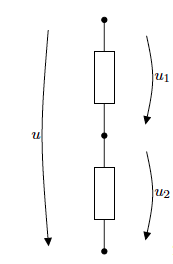
\includegraphics[width=0.19\textwidth]{laborator_01/figuri/divizor_schema_exemplu}
	\caption{Divizorul de tensiune.}
	\label{fig:divizor_schema_exemplu}
\end{figure}

\begin{figure}
	\centering
		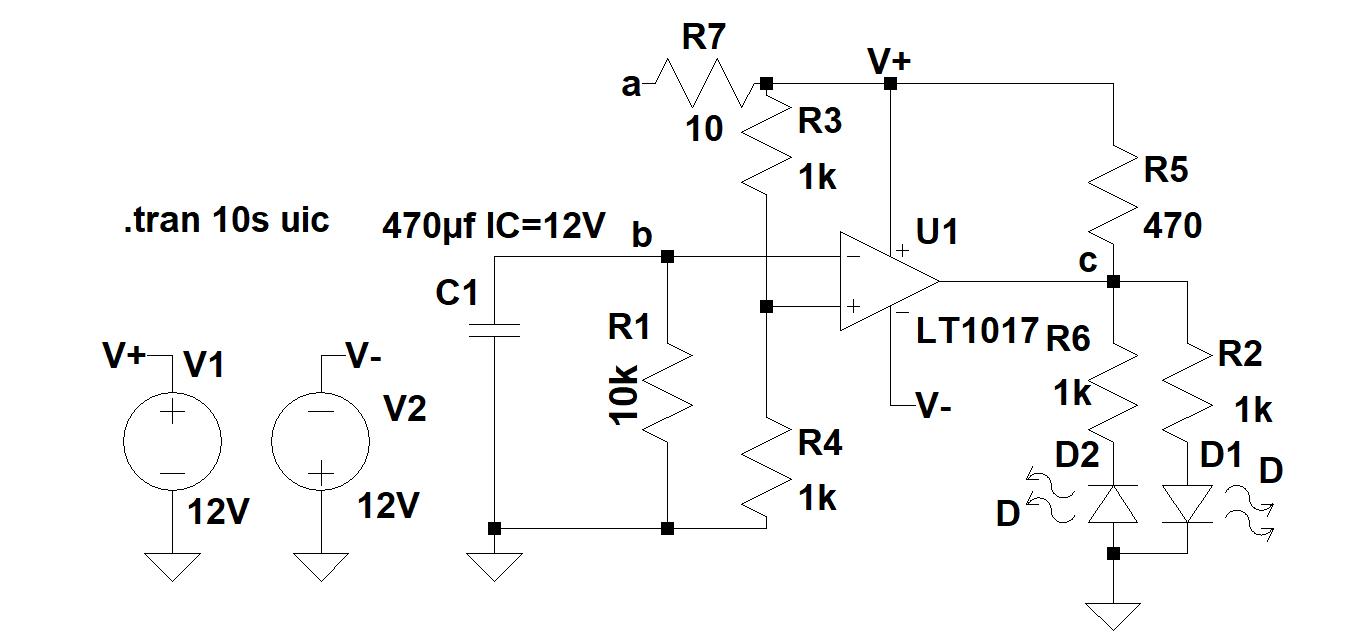
\includegraphics[width=0.8\textwidth]{laborator_01/figuri/comparator_cu_divizor}
	\caption{Circuit comparator cu tensiunea de referin't'a dat'a de un divizor de tensiune format din $R_3$ 'si $R_4$.}
	\label{fig:comparator_cu_divizor}
\end{figure}

\subsection*{Scopul lucr'arii}

Obiectivul acestei lucr'ari de laborator este ilustrarea modului 'in care se 'imbin'a cele trei aspecte ale domeniului Calculelor 'stiintifice 'in inginerie (CSE -- \textit{Computational science and engineering}): conceptele (lumea ideilor), simul'arile (lumea virtual'a) 'si experimentele (lumea real'a). 'In acest scop, exemplele folosite sunt simple din punct de vedere conceptual, tocmai pentru a permite nu numai explicarea aspectelor strict legate de teoria circuitelor, dar 'si eviden'tierea conexiunilor cu teoria sistemelor, metode numerice, analize pe baza simul'arilor 'in SPICE. 
%Aceast'a lucrare de laborator creeaz'a o baz'a solid'a de analiz'a, astfel 'inc\^at trecerea la circuite mai complicate, cu elemente neliniare sau m'arimi variabile 'in timp s'a se fac'a relativ u'sor.

%\subsection*{Concepte teoretice utile}
%
%Pentru a putea efectua cu succes aceast'a lucrare trebuie s'a revede'ti urm'atoarele concepte prezentate la curs: intensitatea curentului electric, tensiunea electric'a, poten'tialul electric, legile lui Kirchhoff, rezistorul dipolar liniar, sursa ideal'a de tensiune. 
%%Pentru a v'a verifica aceste cuno'stin'te completa'ti chestionarul 1 (vezi Anexa 1) de pe moodle.
%
%%\begin{exercise}[Pe moodle, 'inainte de laborator]
%%Efectua'ti chestionarul 1 de pe moodle. 'Incerca'ti s'a ob'tine'ti un punctaj c\^at mai mare.
%%\end{exercise}

